\documentclass[a4paper,11pt]{article}

\usepackage[margin=3cm]{geometry}
\usepackage{amsfonts}
\usepackage{amsmath}
\usepackage{amssymb}
\usepackage{graphicx}

\usepackage[utf8]{inputenc}
%\usepackage[cp1250]{inputenc}
\usepackage[polish]{babel}
\usepackage[T1]{fontenc}

%----------------------
\def\\{\hfill\break}


%----------------------
\title{Projekt Egzaminacyjny}
\author{Maria Koren}
\date{Listopad 2023}



\begin{document}

\maketitle
\newpage
\tableofcontents{}
\newpage

\section{Wstęp}

W tym projekcie reprezentowana jest analiza danych spółki KMR.UK (Kenmare Resources Plc)
\smallskip


\section {Analiza cen spółek}
Kenmare Resources plc to uznana firma wydobywcza, która zarządza kopalnią minerałów tytanu Moma położoną na północno-wschodnim wybrzeżu Mozambiku.
Kopalnia prowadzi produkcję komercyjną od 2009 roku i jest uznawana za głównego dostawcę produktów z piasku mineralnego dla klientów na całym świecie, działających w ponad
15 krajach.

\section{Część 1}

\subsection{Wykres kursów zamknięcia pokazujący zmiany w czasie oraz
histogram}

Zrobiono wykres  kursu zamknięcia pokazujący zmiany w czasie, rysunek \ref{fig:cena_podcaz_zamkn}

\begin{figure}[h]
  \centering
  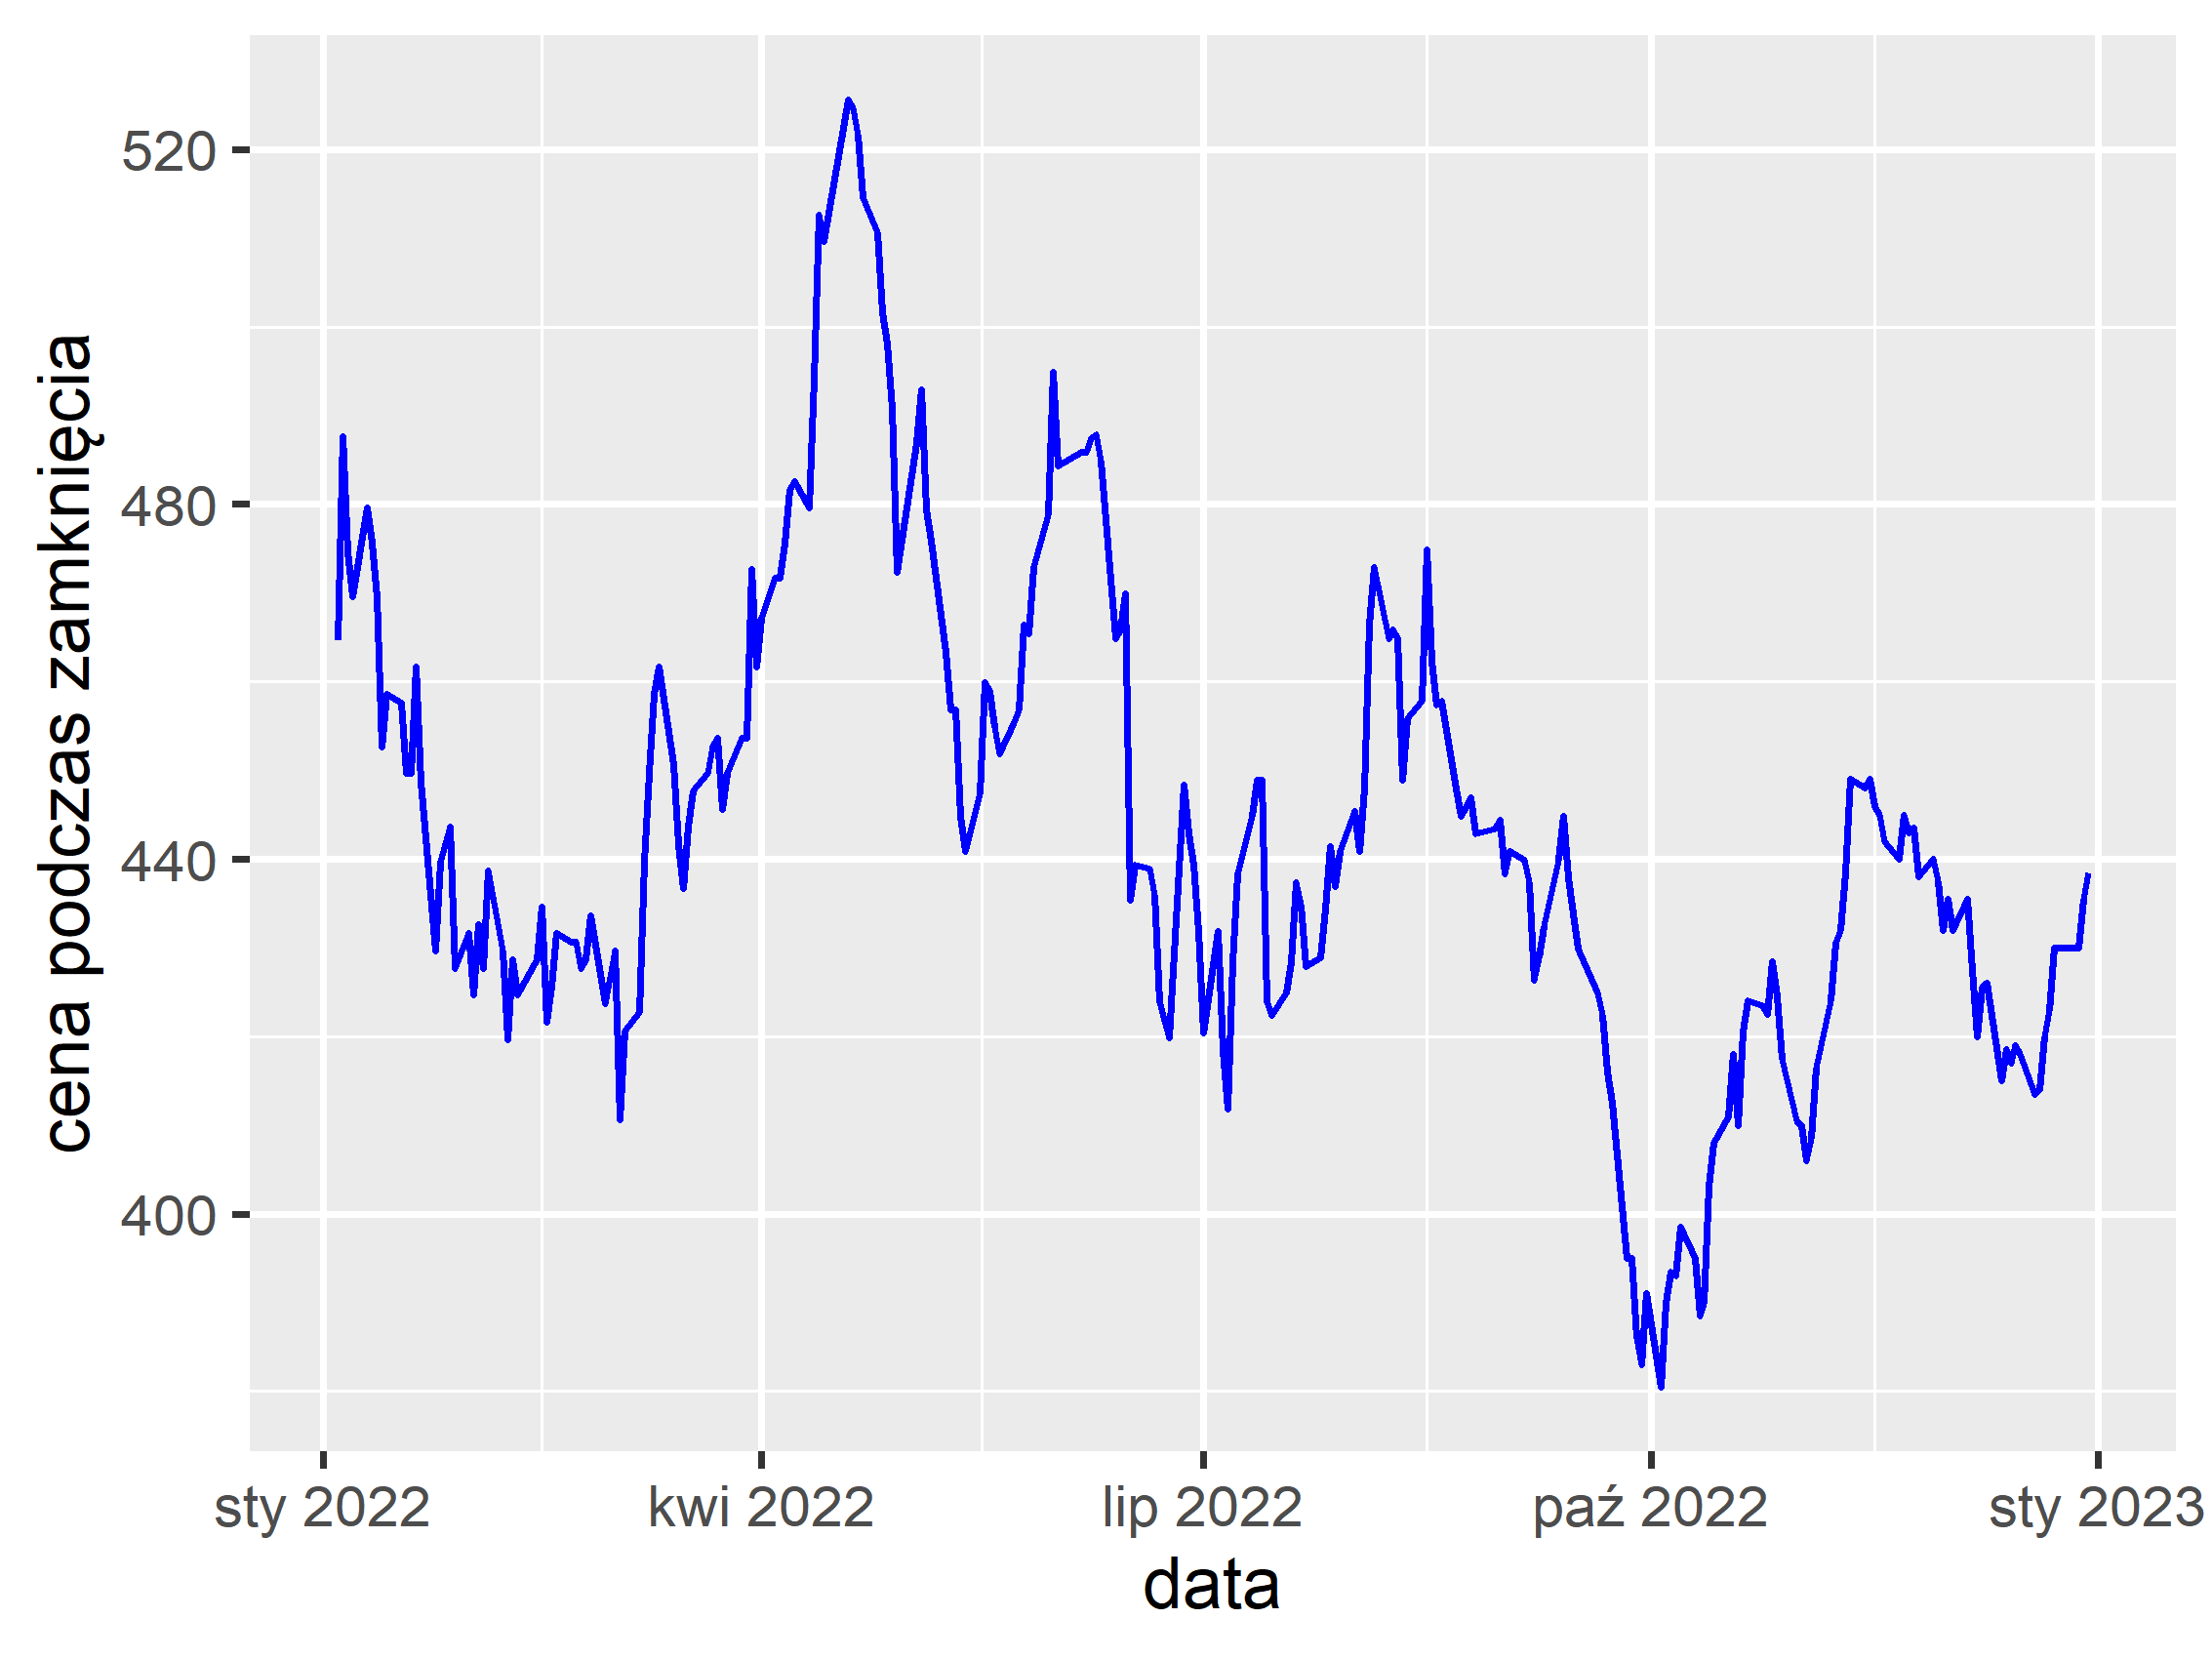
\includegraphics[width=10cm]{cena_poczas_zamkn.png}
  \caption{Cena podczas zamknięcia}
  \label{fig:cena_podcaz_zamkn}
\end{figure}

Oraz histogram, pokazujacy liczebność danych, rysunek \ref{fig:histogram}
\newpage
\begin{figure}[h]
  \centering
  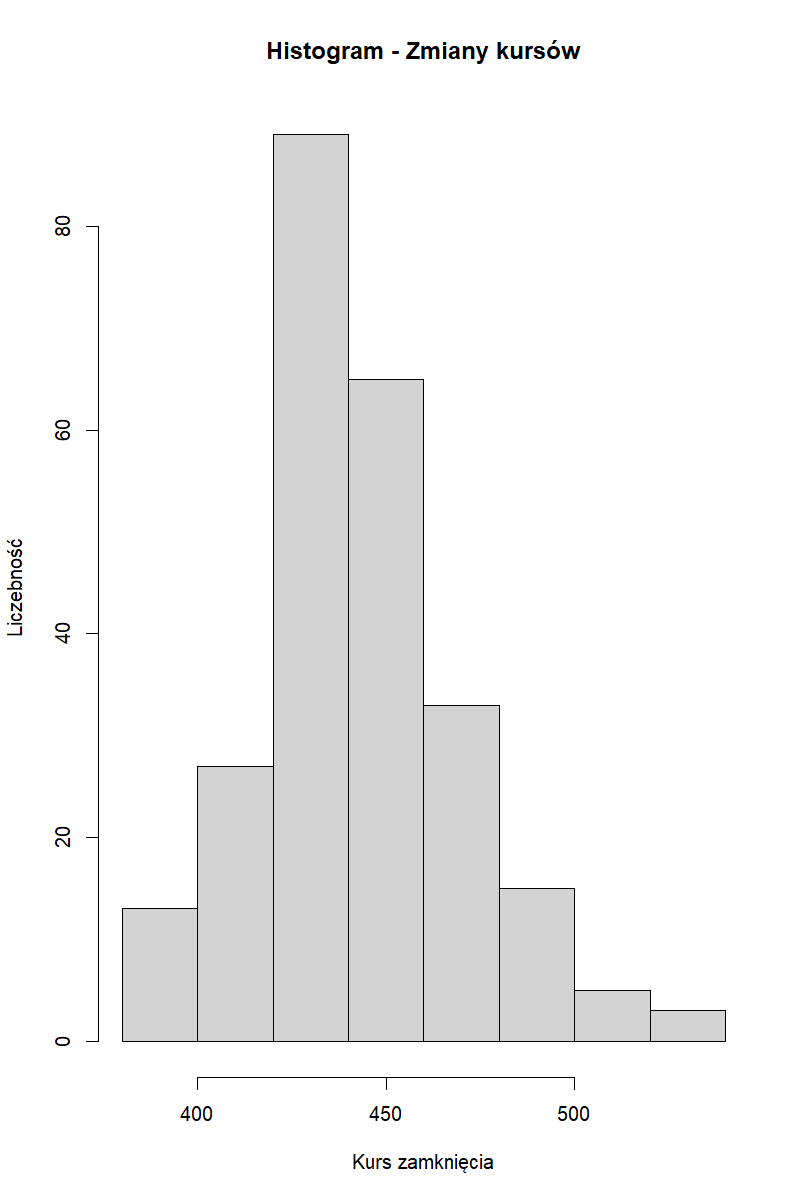
\includegraphics[width=10cm]{histogram.png}
  \caption{Histogram danych}
  \label{fig:histogram}
\end{figure}


\subsection{Statystyki opisowe}

Zostały obliczone nastepujące statystyki opisowe: średnia, odchylenie standardowe, skośność oraz kurtoza

Wyniki statystyk znajdują się w poniższej tabeli \ref{tab:statystyki_opisowe}

\begin{table}[h]
  \centering
  \begin{tabular}{|c|c|c|c|c|}
    \hline
     & $\bar{x}$ & odch. st. & skośność & kurtoza  \\
    \hline
    akcje & 442.8741 & 26.7262 & 3.574323 & 0.52783 \\
    \hline

    \hline
  \end{tabular}
  \caption{Statystyki opisowe}
  \label{tab:statystyki_opisowe}
\end{table}

\subsubsection{Interpretacja wyników}
\begin{itemize}
  \item Otrzymana skośność mówi o przewadzę wartości wyższych (wartość skośności powyżej zera)
  \item  Otrzymana kurtoza mówi cieńszych ogonach niż rozkład normalny (bardziej płaski) (wartość kurtozy mniej niż 3)

\end{itemize}


\subsection{Estymacja parametrów trzech rozkładów korzystając z estymatora największej wiarygodności (MLE)}

Wyestymowano wyniki trzech rozkładów: normalnego, log-normalnego oraz rozkładu Weibulla za pomocą estymatora MLE. Wyżej wymienione wykresy dodano do wcześniejszego histogramu, co widać za rysynku \ref{fig:histogram_wykresy}


\begin{figure}[h]
  \centering
  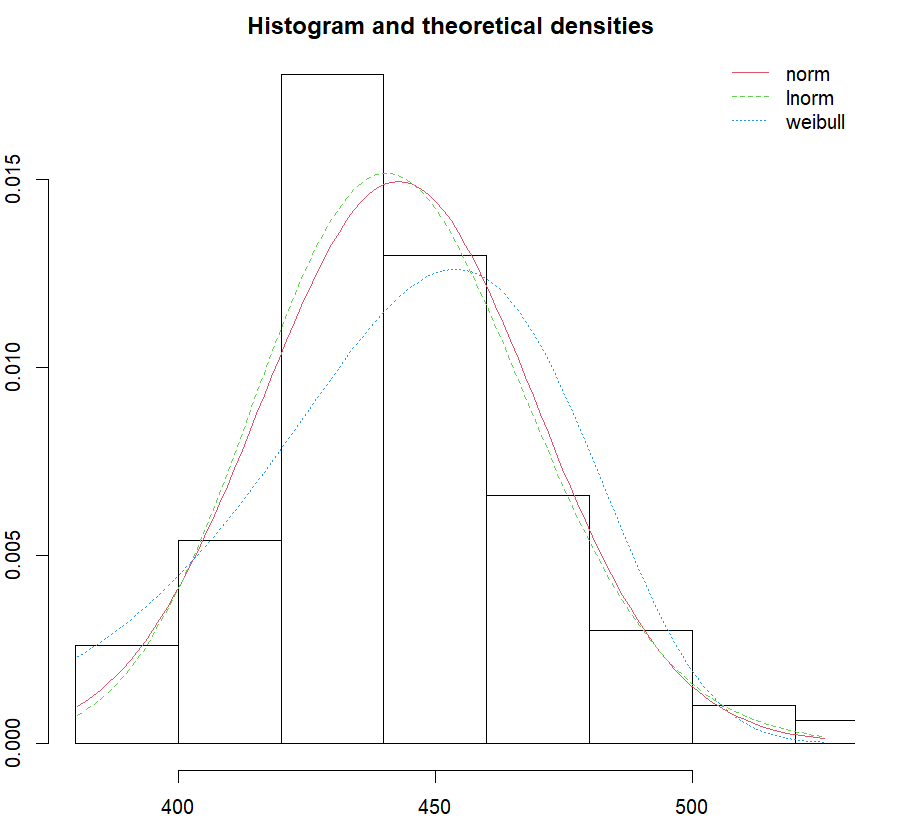
\includegraphics[width=10cm]{histogram_z_wykresami.png}
  \caption{Histogram wraz z estymowanami rozkładami}
  \label{fig:histogram_wykresy}
\end{figure}

Wyniki estymacji parametrów są przedstawione w tabeli \ref{wyniki_estymacji}
\begin{table}[h]
  \centering
  \begin{tabular}{|c|c|c|}
    \hline
     & $\mu$ & $\sigma$   \\
    \hline
    normalny & 442.8741 & 26.67269  \\
    \hline

    \hline
     & $\mu$ & $\sigma$   \\
    \hline
    log-normalny & 6.091499 & 0.05957788  \\
    \hline

    \hline
     & $a$ & $\sigma$   \\
    \hline
    weibulla & 15.61307 & 455.8914  \\
    \hline
  \end{tabular}
  \caption{Wyniki estymacji parametrów}
  \label{wyniki_estymacji}

\end{table}



Te wyniki oznaczają, że zostały dopasowane następujące rozkłady:

\begin{itemize}
  \item $X \sim\ N(442.87, 26.67)$
  \item $X \sim\ LN(6.09, 0.059)$
  \item $X \sim\ W(15.61, 455.89)$

\end{itemize}

\subsection{Wykresy diagnostyczne}
Zostały zrobione wykresy diagnostyczne qq-plot (rysunek \ref{fig:qqplot}) oraz cdf (rysunek \ref{fig:cdf})

\begin{figure}[h]
  \centering
  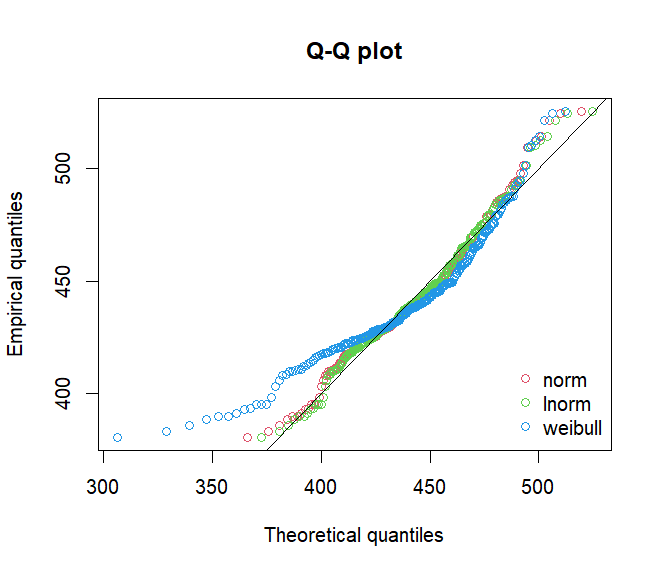
\includegraphics[width=9cm]{qqplot.png}
  \caption{Wykres qq-plot}
  \label{fig:qqplot}
\end{figure}

\begin{figure}[h]
  \centering
  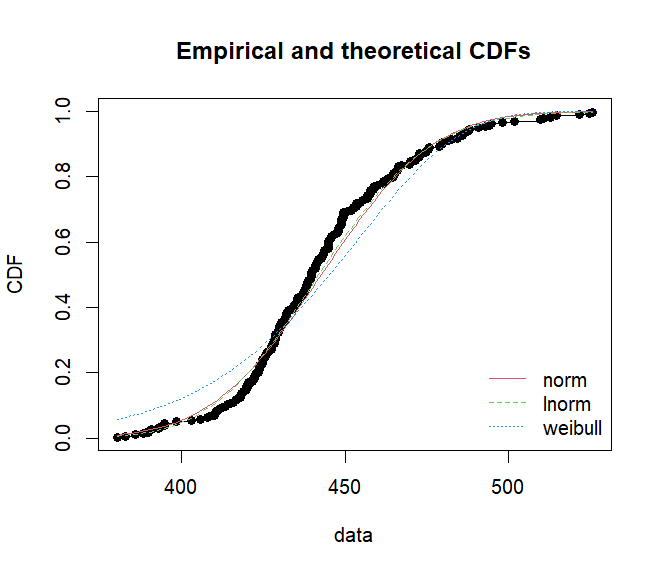
\includegraphics[width=9cm]{cdf.png}
  \caption{Wykres cdf}
  \label{fig:cdf}
\end{figure}

\begin{itemize}
  \item Wykres qq-plot
  
 Jest to wykres kwantyl-kwantyl, na osi pionowej są kwantyle teoretyczne, na osi   poziomowej są kwantyle empiryczne. Kwantyl rzędu $\alpha$  $\in$ (0, 1) zmiennej losowej ciągłej $X$ to taka liczba q, dla której prawdopodobieństwo, że zmienna $X$ przyjmuje   wartości mniejsze lub równe q jest równe $\alpha$.
      
  Najlepiej jest gdy te kwantyle są takie same bądź bardzo blizkie siebie. Dlatego   najlepszym rozkładem  jest najbliższy do prostej $y=x$. W rozważanym przykład takim   jest wykres log-normalny $X \sim\ LN(6.09, 0.059)$
  \item Wykres CDF

  Funkcja rozkładu kumulacyjnego (CDF, Cumulative Distribution Function) to graficzna reprezentacja kumulatywnej dystrybuanty danej zmiennej losowej. CDF dla danej wartości $x$ to prawdopodobieństwo, że zmienna losowa przyjmuje wartość mniejszą lub równą $x$. Czarnym zaznaczone są dane empiryczne. Najlepszym wykresem jest mający teorytyczne dane najbliższe do danych empirycznych. W rozważanym przykładzie takim wykresem jest log-normalny $X \sim\ LN(6.091, 0.059)$
\end{itemize}

Na podstawie wykresów diagnostycznych najlepszym rozkładem jest rozkład logarytmiczno-normalny

\subsubsection{Analiza wartości statystyk KS, CM i AD oraz kryteria informacyjne AIC i BIC}

Bazując wyłącznie na wykresach diagnostycznych, nie jest możliwe wybranie jednego najlepszego wykresu. Dlatego skorzystano ze statystyk Kołmogorowa-Smirnowa, Cramera-von-Misesa, Andersona-Darlinga, a także z kryteriów informacyjnych AIC (Akaike's Information Criterion) oraz BIC (Bayesian Information Criterion)

Wartości ze statystyk KS, CM, AD są umieszczone w tabeli \ref{tab:statystyki}. Wartości kryteriów AIC, BIC w tabeli \ref{tab:kryteriaInf}


\begin{table}[h]
  \centering
  \begin{tabular}{|c|c|c|c|}
    \hline
     & normalny & log-normalny & weibull  \\
    \hline
    Kolmogorov-Smirnov & 0.09168955 & 0.0798396 & 0.138442\\
    \hline
    Cramer-von Mises & 0.3613063 & 0.2485924 & 1.257677 \\
    \hline
    Anderson-Darling & 2.005469 & 1.412547 & 7.416593 \\
    \hline
  \end{tabular}
  \caption{Statystyki}
  \label{tab:statystyki}
\end{table}


\begin{table}[h]
  \centering
  \begin{tabular}{|c|c|c|c|}
    \hline
     & normalny & log-normalny & weibull  \\
    \hline
    Akaike's Information Criterion & 2355.289 & 2348.983 & 2415.692\\
    \hline
    Bayesian Information Criterion & 2362.332 & 2356.026 & 2422.735 \\
    \hline
  \end{tabular}
  \caption{Kryteria informacyjne}
  \label{tab:kryteriaInf}
\end{table}

Ponieważ statystyki są oparte na porównaniu odległości dystrybuant, najlepszym rozkładem jest ten, który jest najbliżej do danych teorytycznych (ma najmniejszą odległość), czyli ma najmniejszą wartość statystyki. W kryteriach informacyjnych za najlepszy rozkład również jest uważany rozkład, mający najmniejszą wartosć kryteria. W rozważanym przykładzie takim rozkładem jest rozkład log-normalny $X \sim\ LN(6.09, 0.059)$

\subsection{Testowanie hipotezy o równości rozkładów, wykorzystując  statystykę KS}

Zrobiona hipoteza H0: $F=LN(6.09, 0.0595)$ przeciwko hipotezie H1: F nie jest rowny $LN(6.09, 0.059)$

Zgenerowano $N=10000$ probek licznosci $n$ (równej ilości danych) z rozkładu $F0=LN(6.09, 0.059)$ wybranego wcześniej jako najlepszego rozkładu i obliczono odleglość dystrybuant empirycznych od rozkladu F0 (wartosc statystyki Dn)

Obliczona również wartość statystyki dla rzeczywustych danych

Rysowany jest histogram statystyk testu KS uzyskanych z danych losowych, a także dodany jest punkt dla statystyki testu KS uzyskanej z rzeczywistych danych dla porównania danych rzeczywistych z danymi losowymi tego rozkładu


\begin{figure}[h]
  \centering
  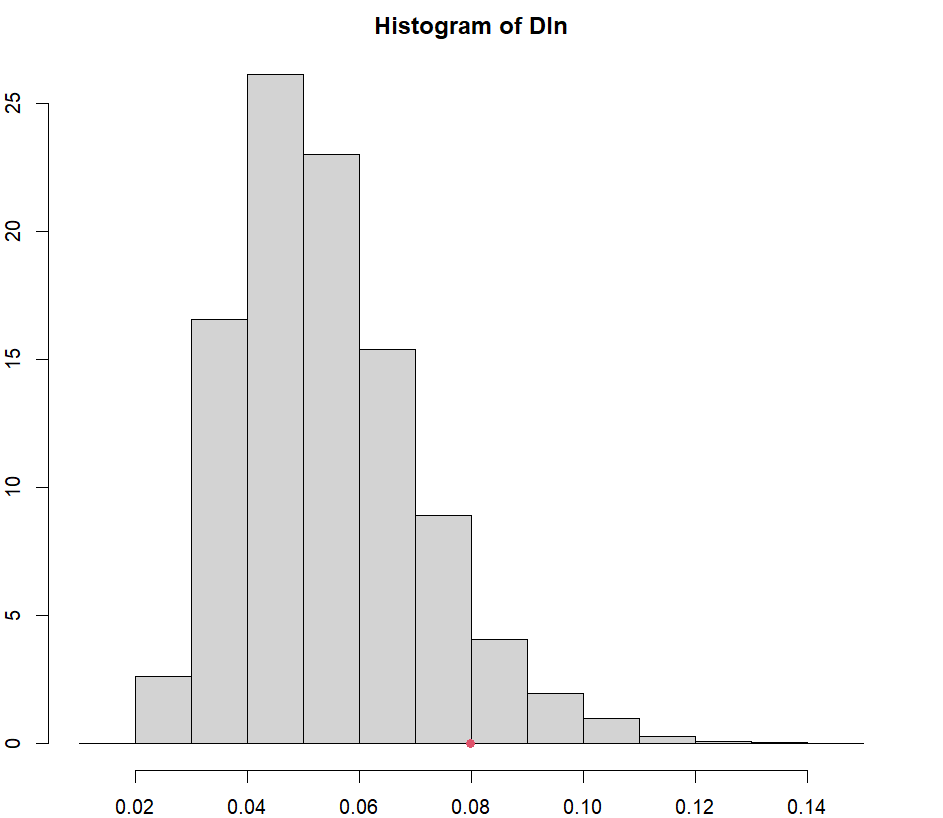
\includegraphics[width=9cm]{histogram_dane_teoryteczne.png}
  \caption{Histogram danych teorytycznych}
  \label{fig:hisT_dane_teor}
\end{figure}

Z wykresu widać, że wynik z danych rzeczywistych jest umieszczony w miejscu, gdzie dane losowe jeszcze są
\\

Ta statystyka zwraca 2 dane: odległość (wartość \textit{statistic}) oraz prawdopodobieństwo że wartości statystyki KS są takie same lub większe, gdy hipoteza zerowa jest prawdziwa

Wyniki tego testowania zostaną umieszczone w tabeli \ref{tab:wyniki_testowania}:

\begin{table}[h]
  \centering
  \begin{tabular}{|c|c|}
    \hline
     statistic & p-value   \\
    \hline
     0.0798396  & 0.0827\\
    \hline
  \end{tabular}
  \caption{Wartość statystyki KS w testowaniu hipotezy}
  \label{tab:wyniki_testowania}
\end{table}


P-wartość informuje o prawdopodobieństwie uzyskania takiej samej lub bardziej ekstremalnej statystyki testu, niż ta, którą otrzymaliśmy z danych rzeczywistych (zakładając że dane pochodzą z tego samego rozkładu)

Ponieważ p-wartosć  p = 0.0827 > 0.05 zatem nie ma powodów odrzucenia hipotezy. Uzyskane wyniki potwierdzają wybraną hipotezę  o logarytmiczno-normalnym $LN(6.09, 0.059)$ rozkładzie naszych danych



\section{Podsumowanie}
Badając dane spólki Kenmare Resources Plc za 2022 rok, wychodzi że dane kursu zamknięcia mieli rozkład logarytmiczno-normalny $LN(6.09, 0.059)$
\end{document}

